\section{Tsiligiridis' Algorithms}

\subsection{Stochastic Algorithm}

\begin{frame}{Tsiligiridis' Algorithms}

	\note<1->{One of the first papers on the OP}
	\note<2->{
		In original paper: Input assumed to be euclidean \begin{itemize}
			\item test instances used are also euclidean
		\end{itemize}
	}
	\note<3->{Will discuss the S algorithm}

	\begin{itemize}
		\item<1-> One of the first papers on the topic \cite{tsiligiridis_heuristic_1984}
		\item<2-> In original paper: Input is Euclidean
		\item<2-> Here: One of his algorithms
	\end{itemize}
\end{frame}

\begin{frame}{Stochastic Algorithm (S-Algorithm)}
	\note<2->{
		Instead of picking the locally \enquote{best} node \begin{itemize}
			\item Weigh each available node by its desirability and pick one randomly
		\end{itemize}
	}
	\note<3->{
		Further away and more valuable nodes are more desirable
	}
	\note<4->{
		We need another parameter $k$ \begin{itemize}
			\item We always only consider the best $k$ nodes when choosing a next node
		\end{itemize}
	}

	\begin{columns}
		\begin{column}{0.6\textwidth}
			\begin{itemize}
				\item<2-> Pick random node based on \enquote{desirability} \begin{itemize}
					\item Depends on the distance and score
				\end{itemize}
				\item<4-> Consider $k \in \mathbb{N}$ most desirable nodes
			\end{itemize}
		\end{column}
		\begin{column}{0.5\textwidth}
			\only<2->{
				\begin{tikzpicture}[vertex/.style={draw, shape=circle}]
					\node[vertex] at (1,0) (0) {O};
					\node<2>[vertex] at (-2,1) (1) {$3$};
					\node<3->[red,vertex] at (-2,1) (1) {$3$};
					\node<3->[draw=none,red,above left=-1mm of 1] (1p) {-};
					\node<2>[vertex] at (-1,-0.5) (2) {$8$};
					\node<3->[blue,vertex] at (-1,-0.5) (2) {$8$};
					\node<3->[draw=none,blue,above left=-1mm of 2] (2p) {+};

					\draw[->] (0) -- (1);
					\draw[->] (0) -- (2);
				\end{tikzpicture}
			}
		\end{column}
	\end{columns}


\end{frame}

\begin{frame}{Example}
	\note<1>[item]{
		Start at the origin \begin{itemize}
			\item Always consider the 3 best nodes
			\item Scores inside the nodes
		\end{itemize}
	}
	\note<1>[item]{
		First step: $10, 6$ and $9$ are the best. \begin{itemize}
			\item We randomly pick $9$
		\end{itemize}
	}

	\note<2>[item]{
		Now we continue like this
	}

	\note<5>[item]{
		Note that this algorithm decides this based on the triangle equality like the example algorithm before.\begin{itemize}
			\item Triangle Inequality
		\end{itemize}
	}

	\centering
	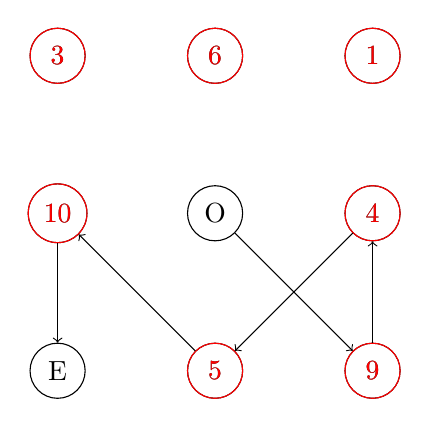
\begin{tikzpicture}
		\node[draw,shape=circle,minimum size=7mm] (origin) at (0,0) {O};
		% left
		\node<5->[draw,shape=circle,minimum size=7mm] (1) at (-2,0) {10};
		\node<1-4>[draw,red,shape=circle,minimum size=7mm] (1) at (-2,0) {10};
		% top left		
		\node<1-3,6->[draw,shape=circle,minimum size=7mm] (2) at (-2,2) {3};
		\node<4-5>[draw,red,shape=circle,minimum size=7mm] (2) at (-2,2) {3};
		% top		
		\node<2,6->[draw,shape=circle,minimum size=7mm] (3) at (0,2) {6};
		\node<1,3-5>[draw,red,shape=circle,minimum size=7mm] (3) at (0,2) {6};
		% right
		\node<1,3->[draw,shape=circle,minimum size=7mm] (4) at (2,0) {4};
		\node<2>[draw,red,shape=circle,minimum size=7mm] (4) at (2,0) {4};
		% bottom
		\node<1,4->[draw,shape=circle,minimum size=7mm] (5) at (0,-2) {5};
		\node<2,3>[draw,red,shape=circle,minimum size=7mm] (5) at (0,-2) {5};
		% bottom right
		\node<2->[draw,shape=circle,minimum size=7mm] (6) at (2,-2) {9};
		\node<1>[draw,red,shape=circle,minimum size=7mm] (6) at (2,-2) {9};
		% top right
		\node<1-4,6->[draw,shape=circle,minimum size=7mm] (7) at (2,2) {1};
		\node<5>[draw,red,shape=circle,minimum size=7mm] (7) at (2,2) {1};
		% bottom left
		\node[draw,shape=circle,minimum size=7mm] (end) at (-2,-2) {E};

		\iffalse
		\node[right=2cm of 7] (b) {$T_{max} = 7$};
		\node[below=1mm of b] (c) {$k = 3$};
		\node[below=1mm of c] (d) {$r = 1$};

		\node<1>[above left=0mm of 1] (1d) {$10$};
		\node<1>[above left=0mm of 2] (2d) {$2.12$};
		\node<1>[above left=0mm of 3] (3d) {$6$};
		\node<1>[above left=0mm of 4] (4d) {$4$};
		\node<1>[above left=0mm of 5] (5d) {$5$};
		\node<1>[above left=0mm of 6] (6d) {$6.36$};
		\node<1>[above left=0mm of 7] (7d) {$0.71$};

		\node<2>[above left=0mm of 1] (1d) {$4.47$};
		\node<2>[above left=0mm of 2] (2d) {$1.06$};
		\node<2>[above left=0mm of 3] (3d) {$2.68$};
		\node<2>[above left=0mm of 4] (4d) {$4$};
		\node<2>[above left=0mm of 5] (5d) {$5$};
		\node<2>[above left=0mm of 7] (7d) {$0.5$};

		\node<3>[above left=0mm of 1] (1d) {$5$};
		\node<3>[above left=0mm of 2] (2d) {$1.34$};
		\node<3>[above left=0mm of 3] (3d) {$4.24$};
		\node<3>[above left=0mm of 5] (5d) {$5$};
		\node<3>[above left=0mm of 7] (7d) {$0.5$};

		\node<4>[above left=0mm of 1] (1d) {$7.07$};
		\node<4>[above left=0mm of 2] (2d) {$1.34$};
		\node<4>[above left=0mm of 3] (3d) {$3$};
		\node<4>[above left=0mm of 7] (7d) {$0.44$};

		\node<5>[above left=0mm of 2] (2d) {$3$};
		\node<5>[above left=0mm of 3] (3d) {$4.24$};
		\node<5>[above left=0mm of 7] (7d) {$0.44$};

		\node<1>[right=2cm of 4] (a) {$T(P) = 0$};
		\node<2>[right=2cm of 4] (a) {$T(P) \approx 1.41$};
		\node<3>[right=2cm of 4] (a) {$T(P) \approx 2.41$};
		\node<4>[right=2cm of 4] (a) {$T(P) \approx 3.82$};
		\node<5>[right=2cm of 4] (a) {$T(P) \approx 5.24$};
		\node<6>[right=2cm of 4] (a) {$T(P) \approx 6.24$};

		\draw<2->[->] (origin) -- node[above] {$\sqrt 2$} (6);
		\draw<3->[->] (6) -- node[right] {$1$} (4);
		\draw<4->[->] (4) -- (5);
		\draw<5->[->] (5) -- node[above] {$\sqrt 2$} (1);
		\draw<6->[->] (1) -- node[left] {$1$} (end);
		\fi

		\draw<2->[->] (origin) -- (6);
		\draw<3->[->] (6) -- (4);
		\draw<4->[->] (4) -- (5);
		\draw<5->[->] (5) -- (1);
		\draw<6->[->] (1) -- (end);
	\end{tikzpicture}
\end{frame}

\begin{frame}
	\frametitle{Generalization}

	\note<1-3>[item]{
		Main point: Trying to drop as many restrictions as feasibly possible \begin{itemize}
			\item So which restrictions does the algorithm rely on
		\end{itemize}
	}
	\note<2-3>[item]{
		Nowhere are uniquely Euclidean features ever required \begin{itemize}
			\item Selecting nodes relies on triangle equality though
		\end{itemize}
	}
	\note<3>[item]{
		Do we really need it? \begin{itemize}
			\item What happens if we drop the triangle inequality
		\end{itemize}
	}
	\note<4>[item] {
		\textbf{Question for the audience:} \begin{itemize}
			\item What would happen on this graph?
		\end{itemize}
	}
	\note<4>[item] {
		Starting at the origin, which nodes can we go to? (Algorithm's perspective) \begin{itemize}
			\item 9? No, since going to 9 and then to the goal would cost $4$
			\item 5? No, since going to 5 and then to the goal would cost $4$
			\item The goal? No, it would cost $5$
		\end{itemize}
	}
	\note<4>[item]{
		Would return, that there is no path \begin{itemize}
			\item Obviously wrong
		\end{itemize}
	}
	\note<5->[item]{
		Seems like there is no trivial way around it \begin{itemize}
			\item Calculate the shortest path to the end for every node? \begin{itemize}
				      \item Might work to an extent
				      \item[!] But shortest paths assume all nodes to be usable
				      \item If some nodes of the paths are already used, the shortest path lengths might increase
			      \end{itemize}
		\end{itemize}
	}

	\begin{columns}
		\begin{column}{0.48\textwidth}
			\begin{itemize}
				\item<2-> Relies on the triangle inequality
				\item<3-> What happens if we drop it? \begin{itemize}
					\item<5-> We can't
				\end{itemize}
			\end{itemize}
		\end{column}
		\begin{column}{0.48\textwidth}
			\includegraphics<3>[width=0.5\textwidth]{res/business_man3_1_question.png}
			\includegraphics<2>[width=0.5\textwidth]{res/business_man2_1_idea.png}
			\includegraphics<5>[width=0.5\textwidth]{res/business_man2_4_think.png}

			\only<4>{
				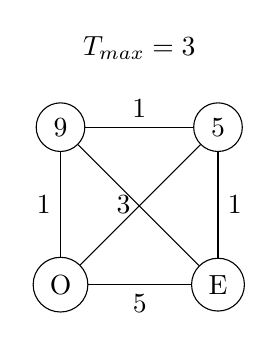
\begin{tikzpicture}[vertex/.style={draw, shape=circle}]
					\node[vertex] at (0,0) (0) {O};
					\node[vertex] at (0,2) (1) {$9$};
					\node[vertex] at (2,2) (2) {$5$};
					\node[vertex] at (2,0) (3) {E};

					\draw (0) -- node[left] {$1$} (1);
					\draw (1) -- node[above] {$1$} (2);
					\draw (2) -- node[right] {$1$} (3);
					\draw (0) -- node[below] {$5$} (3);
					\draw (0) -- node[left] {$3$} (2);
					\draw (1) -- (3);

					\node at (1, 3) {$T_{max}=3$};
				\end{tikzpicture}
			}
		\end{column}
	\end{columns}

\end{frame}